\chapter{Conformal Prediction for Graph Structured Data}
\label{chp:graphConformal}
In the previous chapter, confidence intervals were used to generate online, anytime-valid bounds for the outputs associated with different decision-making models.
However, confidence intervals require a strong assumption on the data-generating distribution at test time i.e, independent and identically distributed (i.i.d) data.
For graph structured data, the edges between different nodes denote potential dependencies between the nodes.
Thus, the i.i.d assumption is violated, and the confidence intervals are no longer valid.
In this chapter, we will discuss conformal prediction, a method that provides valid confidence sets/intervals for graph structured data under a weaker assumption - exchangeability.
While the estimates generated by these are no-longer online, anytime-valid, the strong guarantees provided by these methods can provide a foundation for understanding the uncertainty associated with the predictions in graph structured data.
In this chapter, we will discuss the theoretical underpinnings of conformal prediction and the tradeoffs associated with its application to graph structured data.
%\pmcomment{Maybe move this to appendix}
%Following this, in the second part, we will conclude with a discussion of extending conformal prediction for studying the fairness of decision-making models trained for graph structured data.

%\section{Understanding the Tradeoffs in Graph Conformal Prediction}

Conformal prediction has become increasingly popular as a method for quantifying the uncertainty associated with machine learning models. 
The computational efficiency of the inductive approach has made it the method du jour for building new methods for conformal prediction.
Recent work in graph uncertainty quantification has built upon this approach for conformal prediction on graphs.
The nascent nature of these explorations has lead to conflicting choices for implementations baselines and evaluation of approaches.
We critically analyze the choices made and describe the tradeoffs associated with existing graph conformal prediction work. 
Our theoretical and empirical results provide the rationale for our recommendations for future scholarship in graph conformal prediction.

\section{Introduction}
Modern machine learning models trained on losses based on point predictions are prone to be overconfident in their predictions~\citep{guo2017calibration}. 
The Conformal Prediction (CP) framework~\citep{vovk2005algorithmic} provides a mechanism for generating statistically sound post hoc prediction sets (or intervals, in case of continuous outcomes) with coverage guarantees under mild assumptions.
The usual assumption made in CP is that data are exchangeable, i.e, the joint distribution of the data is invariant to permutations of the data points.
The guarantees provided by CP are distribution-free, and can be added post hoc to arbitrary, black-box predictor scores.
This makes CP an ideal candidate for quantifying uncertainty in complex models, such as neural networks.

Network-structured data such as social networks, transportation networks, and biological networks are ubiquitous in modern data science applications.
Graph Neural Networks (GNNs) have been developed to model vector representations of such network-structured data, and have been shown to be effective in a variety of tasks such as node classification, link prediction, and graph classification~\citep{hamilton2020graph, wu2022graph}.
Uncertainty quantification approaches built for independent and identically distributed (iid) data cannot directly be applied to graph data, as the network structure introduces dependencies between the data points.
However, recent work~\citep{clarkson2023distribution,zargarbashi23conformal,huang2024uncertainty} has demonstrated that in certain settings, CP can be applied to graph data to generate statistically sound prediction sets for the node classification task.

Variations of CP include full CP~\citep{vovk2005algorithmic} which has significant computational cost as the score function must be recomputed with replacement for each data point within the calibration set.
Additionally, cross-conformal prediction~\citep{vovk2015cross}, CV+/Jackknife+~\citep{barber2021predictive} are other variations of CP which are computationally more efficient than full CP, but less efficient than split CP.
Prior work in CP on graphs has mainly focused on the split CP setting due to its computational efficiency, ease of implementation, and distribution-free guarantees with black-box models. 
We focus on split CP in this work.
There is a lack of consensus for the choice and setup of baselines, splitting of common datasets, and evaluation metrics for methods.
In this work, we aim to analyze the choices made by existing work and understand the trade offs associated with these choices.
%In addition, we create a python library which implements different variations of these approaches which would help standardize practices in the evaluation of CP for graph data.


\section{Conformal Prediction}
Conformal prediction is used to quantify the uncertainty of a model by providing prediction sets/intervals with coverage guarantees.
We will focus on conformal prediction in the classification setting.
Given a calibration dataset $\gD_{\text{calib}} = \{(\vx_i, y_i)\}_{i=1}^n$, where $\vx_i \in \gX = \R^d$ and $y_i \in \gY = \{1, \dots, K\}$, conformal prediction can be used to construct a prediction set $C$ such that
\begin{align*}
    \Pr\left[y_{n+1} \in C(\vx_{n+1}) \right] \geq 1 - \alpha
\end{align*}
where $1 - \alpha \in [0, 1]$ is a user-specified coverage level.
The only assumption required for the coverage guarantee is that $\gD_{\text{calib}} \cup \{(\vx_{n+1}, y_{n+1})\}$ is exchangeable.
The following theorem provides a general recipe for constructing a prediction set with coverage guarantee.
\begin{theorem}[\citet{vovk2005algorithmic}]
    Suppose $\{(\vx_i, y_i)\}_{i=1}^{n+1}$ are exchangeable, $s: \gX \times \gY \rightarrow \R$ is a score function, and $\alpha \in [0, 1]$ is a target significance level.
    Let $\hat{q}(\alpha) = \text{Quantile}\left(\frac{\ceil{(n+1)(1-\alpha)}}{n}; \{s(\vx_i, y_i)\}_{i=1}^{n}\right)$
    Define $C_{\alpha}(X) = \{y \in \gY: s(\vx, y) \leq \hat{q}(\alpha)\}$.
    Then,
    \begin{align}
        1 - \alpha +\frac{1}{n+1} \geq \Pr\left[y_{n+1} \in C_{\alpha}(\vx_{n+1}) \right] \geq 1 - \alpha
        \label{eq:CP:coverage}
    \end{align}
    \label{thm:CP:coverage}
\end{theorem}

While Theorem~\ref{thm:CP:coverage} does not place any restrictions on the choice of the score function, the choice of the score function can have a significant impact on the size of the prediction set.
$s$ is usually called the non-conformity score function which measures the degree of non-agreement between the input $\vx$ and the label $y$ i.e., larger scores indicate worse agreement between $\vx$ and $y$.
Note that the setup of theorem~\ref{thm:CP:coverage} is called split CP, which is a special case of CP.
Further, it only provides a marginal coverage guarantee.
\pmcomment{discuss the difference between marginal and conditional coverage and requirements for conditional coverage. Additionally, discuss beta distribution?}



%\section{Applying Conformal Prediction to Graph Structured Data}
\section{Node Classification and Conformal Prediction in Graphs}
The usual tasks of interest in graph data are node classification, link prediction, and graph classification. 
In this work, we focus on node classification and its extensions to conformal prediction.
Consider an attributed homogeneous graph $\gG = (\gV, \gE, \mX)$, where $\gV$ is the set of nodes, $\gE$ is the set of edges and $\mX$ is the set of node attributes.
Let $\mA$ denote the adjacency matrix for the graph.
Further, let $\gY = \{1, \dots, K\}$ denote set of class labels associated with the nodes.
For $v \in \gV$, $\vx_v \in \R^d$ denotes its features and $y_v \in \{1, \dots, K\}$ denotes the corresponding class label.
The task of node classification is to learn a model $F: \gX \to Y$ which predicts the label for each node given node features as input.
Corresponding to the CP partitions, we denote the nodes in the training set as $\gV_{\text{train}}$, validation set as $\gV_{\text{valid}}$, calibration set as $\gV_{\text{calib}}$, and test set as $\gV_{\text{test}}$.
We denote $\gV_d = \gV_{\text{train}} \cup \gV_{\text{valid}}$ 
as the development set of the base model (non-conformalized). 
Note that labels are available only for nodes in the train, validation and calibration sets, and must be predicted for the test set.
The model cycle will involve four phases, viz. training, validation, calibration, and testing.
Next, we discuss the different settings for node classification in graphs and the applicability of conformal prediction.

\noindent \textbf{Transductive setting}
In this setting, the model has access to the fixed graph $\gG$ during training, validation, calibration, and testing.
However, the labels associated with the test nodes $\gD_{\text{test}}$ are unknown. 
%We assume that $\gV_{\text{test}} \cap \gV_{\text{calib}}$ are exchangeable.
We designate a fixed set of nodes disjoint from the training and validation set as  $\gV_{\text{test}} \cup \gV_{\text{calib}}$ and then randomly sample nodes from this set to form $\gV_{\text{calib}}$ and $\gV_{\text{test}}$.
This is the setting considered in~\citet{zargarbashi23conformal} and~\citet{huang2024uncertainty}.
Note that the labels for the calibration nodes are not available for training/validation of the base model, though the neighborhood information $(\gV, \gE)$ and the features $\vx_v$ and labels $y_v$, $v \in \gV_d$ are available.
During the calibration phase, the features and labels for the calibration nodes, along with the neighborhood information, are used to compute the non-conformity scores.
This split ensures that the base model cannot distinguish between the calibration and test nodes, and hence exchangeability holds for $v \in \gV_{\text{calib}} \cup \gV_{\text{test}}$.

\noindent \textbf{Inductive setting}
We briefly describe the inductive setting and note that the exchangeability assumption will be violated in this setting (in general).
The base model is provided with the graph induced by the development nodes only $(\gV_d, \gE_d, \mX_d)$.
In the calibration/test phases, the nodes arrive either one at a time or in batches.
Thus, nodes arriving later in the sequence will have access to neighbors that arrived earlier, breaking the exchangeability assumption.

In line with previous work, we focus on the transductive setting.
The following theorem shows that in the transductive setting, a score model trained on the calibration set will generate scores exchangeable with the test set, and thus allow the use of conformal prediction in the transductive setting.

\begin{theorem}[\citet{zargarbashi23conformal,huang2024uncertainty}]
    Let $\gG = (\gV, \gE, \mX)$ be an attributed graph, and $\gV_{\text{calib}} \cup \gV_{\text{test}}$ be exchangeable.
    Let $F: \gX^{|V|} \rightarrow \Delta^{|V| \times K}$ be any permutation equivariant model on the graph (for instance, GNN). 
    Define $F(G) = \Pi \in \Delta^{|V| \times K}$ be the output probability matrix for a model trained on only $\gV_d$.
    Then any score function $s(v, y) = s(\Pi_v, y, \gG)$ is exchangeable for all $v \in \gV_{\text{calib}} \cup\gV_{\text{test}} $
    %Let $F: \gX \to \Delta_{\gY}$ be a model trained on $\gV_{\text{train}} \cup \gV_{\text{valid}}$.
    %Let $\hat{F}: \gX \to \Delta_{\gY}$ be a model trained on $\gV_{\text{calib}}$.
    %Then, the scores $\hat{F}(\vx)$ are exchangeable with $F(\vx)$ for $\vx \in \gV_{\text{test}}$.
    \label{thm:exchangeability}
\end{theorem}
The intuition for this theorem is that if the output of the permutation equivariant function (e.g., GNN) $F$ does not depend on the order of the nodes in the graph (for e.g. GNN output depends on the neighbors, not the order of the nodes), then the outputs of the GNN will also be exchangeable.
The formal proof for this theorem is available in~\citet{zargarbashi23conformal,huang2024uncertainty}.
This theorem paves the way for using conformal prediction for transductive node classification in graphs.
%\pmcomment{TODO: thm and proof for all scores}

%\pmcomment{Exchangeability for transductive, and potential for inductive}

%\subsubsection{Node Classification}
%Let $f: \gX \to \R_K$ denote the class wise scores associated with a node classification model trained on a separate split of the data ($\gD_{\text{train}}$).
%For example, these could be the pre-final output layer of a graph neural network (either before or after softmax normalization).
%and a trained model with classwise prediction the goal is to learn a model $\pi: \gX \to \Delta_K$, where $\Delta_K$ is the $K$-dimensional probability simplex.
%
%\pmcomment{below text optionol}
For the following sections, we will assume that the base model $\hat{\pi}: \gX \to \Delta_{\gY}$, where $\Delta_{\gY}$ is the probability simplex over the elements of $\gY$ and is learned using the training and validation sets $\train \cup \valid$. 
The calibration set $\calib$ is used to determine the $\hat{q}(\alpha)$ from Theorem \ref{thm:CP:coverage} and the test set $\test$ is the set for which we want to compute our prediction sets.
In general, the outputs $\hat{\pi}$ need not lie over a simplex; they can be in $\R^K$.
However, this greatly simplifies the exposition for the following sections and is the standard practice in prior work.



\section{Conformal Scores for Graphs: Choices and Tradeoffs}
In this section, we critically examine some decisions made in the implementations of existing graph conformal prediction work.
We discuss the trade-offs associated with these choices and provide recommendations for future scholarship in graph conformal prediction.

\subsection{Dataset Splits and Training}
There are several methods of partitioning the data to generate the different partitions of the sets. 
Two methods which are used in other works on graph conformal prediction for classification are (1) full-split paritioning~\cite{huang2024uncertainty} and (2) label-based sample partitioning~\cite{zargarbashi23conformal}.
%\avcomment{Add citations for methods that use each one} %These methods originate from works that consider the classification task in either a supervised or semi-supervised setting, respectively.
 
\noindent \textbf{Full-Split (FS) Paritioning}
In this case, the data is split such that each subset of the partition adheres to a size constraint defined in terms of a percentage/fraction of the full node set $\gV$.
For example, in CF-GNN \cite{huang2024uncertainty} the authors split the datasets in their experiments randomly, but adhering to a $20\%/10\%/35\%/35\%$ split of $\train/\valid/\calib/\test$, respectively.
Note that the overall percentage of data for which we do provide labels (in either the development or calibration set) is a large proportion ($65\%$) of the full dataset.
For non-conformal score models with numerous trainable parameters, this splitting scheme is ideal as it allows for a large amount of data to be used for training the calibration score  model.
We explore the following splitting schemes under FS partitioning:
($\train,\valid,\calib,\test$) = ($0.2, 0.1,0.35, 0.35$), ($0.2,0.2,0.3,0.3$), ($0.3,0.1,0.3,0.3$), and ($0.3,0.2,0.25,0.25$).

\noindent \textbf{Label-Count (LC) Sample Partioning}
In this splitting scheme, the data is split to ensure an equal number of samples for each class/label are present in the train, validation, and calibration set.
The remaining nodes are then used for the test set.
Such settings are common in  settings where only a small proportion of training/labeled nodes are available, such as in semi-supervised learning.
This setting is ideal for methods that do not have a large number of parameters to train.
We explore setting the number of samples per class to 10, 20, 40, and 80.
Note that we assign nodes for each class into train, validation, calibration, and test sets sequentially, so it is feasible in this setup to have some classes having no representative samples in some partitions. 


\subsection{On TPS and Adaptability}
Threshold Prediction Sets (TPS)~\citep{sadinle2019least} is a simple technique for generating conformal prediction sets.
The score function $s(\vx, y) = 1 - \hat{\pi}(\vx)_y$ directly maps the probability from the base model for the correct class into a non-conformity score.
The score is higher if the model has a lower probability assigned to the correct class, indicating the label is less conforming with the model.
A $1-\alpha$ (approximate) quantile creates a probability inclusion threshold for this score over the calibration set ensures coverage and can be shown to generate prediction sets with the smallest expected size~\cite{sadinle2019least}.
However, the TPS score has been known to undercover hard examples and overcover easy ones~\citep{angelopoulos2021uncertainty,zargarbashi23conformal} to achieve this efficiency.
Here, hard/easy refers to the coverage achieved by the prediction set in relation to the prediction set size.
By overcovering easy examples, TPS can still maintain the overall coverage guarantee without having to correctly account for coverage over harder examples.

We note that this discrepancy is claimed to occur as the TPS scores are not `adaptive' and consider only one dimension of the score for each calibration sample.
However, \citet{sadinle2019least} also proposed a labelwise control version of TPS.
Instead of defining a single threshold for all classes, they separately compute the threshold for each class and a corresponding $\alpha$.
Thus, they define classwise quantile thresholds as
\[
    \hat{q}(\alpha, y_j) = \text{Quantile}\left(\frac{\ceil{(n+1)(1-\alpha)}}{n}; \braces{s(\vx_i, y_i)\, {i=1, \dots, n, y_i = y_j}}\right)
\]
and the corresponding prediction sets as
\[
    C_{\text{TPS}}(\vx) = \{y \in \gY: s(\vx, y) \leq \hat{q}(\alpha, y)\}
\]
Note that this version would provide coverage for each class label, making it more `adaptive'.
The version defined by \citet{sadinle2019least} allows controlling $\alpha_y$ for each class label, though, for simplicity, we set $\alpha_y = \alpha$ for label-adaptability.
The tradeoff here is that we have fewer calibration samples used for each quantile threshold dimension, which may lead to higher variance in the distribution of coverage~\cite{vovk2012conditional}.
We call this variation of TPS as TPS-Classwise, and consider it in our baselines for comparison.

\subsection{APS and Randomized Sets}
The most popular baseline in work on graph conformal prediction is adaptive prediction sets (APS). 
%\pmcomment{TODO: Include a bunch of papers that use APS as a baseline}
\citet{romano2020classification} introduce APS by defining an optimal prediction set construction mechanism under oracle probability.
Suppose we estimate a prediction function $\hat{f}$ that correctly models the oracle probability $\Pr[Y=y|X_{test}=\vx] = \pi_y(\vx)$ for each $y \in \gY = \{1, \dots, K\}$ 
Let $\pi_{(1)}(\vx), \dots, \pi_{(K)}(\vx)$ be the sorted probabilities in descending order.
For any $\tau \in [0, 1]$, define the generalized conditional quantile funciton at $\tau$ as
\begin{align}
    L(x; \pi, \tau) =  \min\left\{ k \in \{1, \dots, K\}, \sum\limits_{j=1}^k \pi_{(j)}(\vx) \geq \tau \right\}
    \label{eq:APS:L}
\end{align}
Then the corresponding prediction set, $C_\alpha^{\text{or}}(\vx)$ can be constructed from the probabilities needed to reach $1-\alpha$ coverage.
\[
    C_\alpha^{\text{or}}(\vx) = \{y \in \gY: \pi_y(\vx) \geq \pi_{(L(\vx; \pi, 1-\alpha))}(\vx)\}
\]
where $\text{or}$ indicates the usage of the oracle probability.
Further, they define tighter prediction sets in a randomized fashion using an additional uniform random variable $u \sim \text{Uniform}(0, 1)$ as a parameter to construct a generalized inverse. 
This idea draws upon the idea of uniformly most powerful tests in the Neyman-Pearson lemma for level-$\alpha$ sets~\cite{neyman1933ix}.
%\pmcomment{cite, potentially link to Karlin-Rubin}. 
Define
%\pmcomment{$\leq$ vs $<$ and its effect on proof}
\begin{align}
    S(\vx, u; \pi, \tau) = \begin{cases}
        \{y \in \gY: \pi_y(\vx) > \pi_{(L(\vx; \pi, \tau))}(\vx)\} & u < V(\vx; \pi, \tau) \\
        \{y \in \gY: \pi_y(\vx) \geq \pi_{(L(\vx; \pi, \tau))}(\vx)\} & \text{otherwise}
    \end{cases}
    \label{eq:APS:S}    
\end{align}
i.e., the class at the $L(\vx; \pi, \tau)$ rank is included in the prediction set with probability $1 - V(\vx; \pi, \tau)$, where
\[
V(\vx; \pi, \tau) = \frac{1}{\pi_{(L(\vx; \pi, \tau))}(x)} \left\{ \left[\sum\limits_{j=1}^{L(\vx; \pi, \tau)}{\pi_{(j)}(x)} \right] - \tau \right\}
\]
The corresponding randomized prediction sets are $C_\alpha^{\text{or}}(\vx) = S(\vx, U; \pi, 1 - \alpha)$, $U \sim U(0, 1)$
Note that in general, the coverage guarantees provided in conformal prediction hold only in expectation over the randomness in $(\vx_i, y_i), i = 1, \dots, n+1$.
The randomized prediction sets continue to provide the guarantee with additional randomness over $u_i$.
To make this work for a non-oracle probability $\hat{\pi}(\vx)$, they define a non-conformity score $A$
\begin{align}
    A(\vx, y, u;\hat{\pi}) = \min\{\tau \in [0, 1]: y \in S(\vx, u; \hat{\pi}, \tau)\}
    \label{eq:APS:score}
\end{align}

Assume that $\hat{\pi}$ are all distinct - for ease of defining rank.
Suppose the rank of the true class amongst the sorted $\hat{\pi}$ be $r_y$, i.e., $\sum\limits_{i=1}^K \1[\hat{\pi}_i(\vx) \geq \hat{\pi}_{y}] = r_y$
Solving for $\tau$ as a function of $\hat{\pi}$  (see Appendix~\ref{appx:APS:tau}, for proof),
\begin{align}
A(\vx, y, u;\hat{\pi}) = \left[ \sum\limits_{i=1}^{r_y} \hat{\pi}_{(i)}(\vx) \right] - u \hat{\pi}_{y}
\end{align}

Instead, if a deterministic set is used to define the conformal score instead (i.e., the randomized set construction is not carried out), then we could just add the probabilities until the true class is included:
\begin{align}
    \Tilde{A}(\vx, y;\hat{\pi}) = \left[ \sum\limits_{i=1}^{r_y} \hat{\pi}_{(i)}(\vx) \right]
\end{align}
This version of APS still provides the same conditional coverage guarantees and has a simpler exposition as the prediction sets are constructed by greedily including the classes until the true label is included.
 Thus, this version is provided as the implementation in the popular monographs on conformal prediction by~\citet{angelopoulos2021gentle, angelopoulos2023conformal}.
However, the lack of randomization may sacrifice on the efficiency. 
This modification of score affects both the quantile threshold computation during the calibration phase and the prediction set during the test phase.
We will now show the conditions that impact the efficiency more formally.
Let 
\[
    \hat{q}_{A} = \text{Quantile}\left(\frac{\ceil{(n+1)(1-\alpha)}}{n}; \{A(\vx_i, y_i, u_i; \hat{\pi})\}_{i=1}^{n}\right)
\]
and
\[
    \hat{q}_{\Tilde{A}} = \text{Quantile}\left(\frac{\ceil{(n+1)(1-\alpha)}}{n}; \{\Tilde{A}(\vx_i, y_i; \hat{\pi})\}_{i=1}^{n}\right)
\]
Define $A_i(y) := A(\vx_i, y, u_i; \hat{\pi})$ and $\Tilde{A}_i(y) := \Tilde{A}(\vx_i, y, u_i; \hat{\pi})$. From the definition of the prediction sets and non-conformity scores, we have 
\[
    C_A(\vx_{n+1}) = \{y \in \gY: A_{n+1}(y) \leq \hat{q}_{A}\}
\] and 
\[
    C_{\Tilde{A}}(\vx_{n+1}) = \{y \in \gY: \Tilde{A}_{n+1}(y) \leq \hat{q}_{\Tilde{A}}\}
\] 
denote the prediction sets corresponding to the two score functions (with and without randomization).
Define $C_{A}^{i} = C_{A}(\vx_{i})$. 
Let $y'_i \in \{1, 2, \dots, K\} \setminus \{y_i\}$ be any incorrect class label for each $\vx_i$.
Define 
\[
    \alpha_c^A \in [0, 1], \hat{q}_A \widetilde{=} \text{Quantile}\left( \frac{\ceil{(n+1)(1 - \alpha_c^A)}}{n}; \{A(\vx_i, y'_i, u_i; \hat{\pi})\}_{i=1}^n \right)
\]
\[
    \alpha_c^{\Tilde{A}} \in [0, 1], \hat{q}_{\Tilde{A}} \widetilde{=} \text{Quantile}\left( \frac{\ceil{(n+1)(1 - \alpha_c^{\Tilde{A}})}}{n}; \{A(\vx_i, y'_i, u_i; \hat{\pi})\}_{i=1}^n \right)
\]    
as the thresholds for which the corresponding quantile of the scores for the correct classes $A_i(y_i)$ and $\Tilde{A}_i(y_i)$ achieve $1-\alpha$ coverage.
Then from the exchangeability of $A(\vx_i, y'_i, u_i; \hat{\pi})$
\[
    1 - \alpha_c^A \leq \Pr[y'_{n+1} \in C_{A}^{n+1}] \leq 1 - \alpha_c^A + \frac{1}{n+1}
\]
and similarly, from the exchangeability of $\Tilde{A}(\vx_i, y'_i, u_i, \hat{\pi})$
\[
    1 - \alpha_c^{\Tilde{A}} \leq \Pr[y'_{n+1} \in C_{\Tilde{A}}^{n+1}] \leq 1 - \alpha_c^{\Tilde{A}} + \frac{1}{n+1}
\]
We will show that as long as these thresholds are sufficiently separated, the randomized prediction set will be more efficient than the non-randomized one. 

\begin{theorem}
Assume that $\alpha_c^A - \alpha_c^{\Tilde{A}} \geq \frac{2}{n+1}$ then prediction set constructed using randomization is more efficient than without. Formally, 
\[
    \E\left[|C_{\Tilde{A}}(\vx_{n+1})| - |C_A(\vx_{n+1})|\right]  \geq 0
\]   
\label{them:APS:efficiency}
\end{theorem}
\begin{proof}
Consider the case with only two potential class labels $K = \{1, 2\}$. 
%Let $\Pr[y_{n+1} = 1] = \eta = 1 - \Pr[y_{n+1} = 2]$.

%From the definition of $C_A^i$
%\[
%    \alpha_c = \min\left\{\alpha \in [0, 1] : \hat{q}_A \leq \text{Quantile}\left( \frac{\ceil{(n+1)(1 - \alpha)}}{n}; \{A(\vx_i, y'_i, u_i; \hat{\pi})\}_{i=1}^n \right)\right\}
%\]    
%\pmcomment{Such an $\alpha$ may not exist.}
We have
\begin{align*}
    \E\left[|C_{A}^{n+1}|\right] &= \E\left[\sum\limits_{i=1, 2}\1[i \in C_{A}^{n+1})]\right] \\
                                 &= \E\left[\1[y_{n+1} \in C_{A}^{n+1})]\right] + \E\left[\1[y'_{n+1} \in C_{A}^{n+1})]\right]  & \text{linearity}\\
                                 &= \Pr[y_{n+1} \in C_{A}^{n+1}] + \Pr[y'_{n+1} \in C_{A}^{n+1}] & \text{$\E[\1[A]] = \Pr[A]$}\\
                                 &\leq 1 - \alpha + 1 - \alpha_c^A + \frac{2}{n+1} & \text{(Exchangeability, Theorem~\ref{thm:CP:coverage})} 
\end{align*}
From a similar argument, we can show that 
\[
    \E\left[|C_{\Tilde{A}}^{n+1}|\right] \geq 1 - \alpha + 1 - \alpha_c^A
\]
Thus, 
\begin{align}
    \E\left[|C_{\Tilde{A}}^{n+1}| - |C_{A}^{n+1}|\right] &\geq 1 - \alpha + 1 - \alpha_c^{\Tilde{A}} - \left(1 - \alpha + 1 - \alpha_c^A + \frac{2}{n+1} \right)\\
    &= \alpha_c^A - \alpha_c^{\Tilde{A}} - \frac{2}{n+1}
\end{align}
which is equivalent to our assumption, and this completes the proof.
For $K$ classes, 
\begin{align*}
    \E\brackets{\abs{C_{A}^{n+1}}} &= \Pr[y_i \in C_{A}^{n+1}] + (K-1)\sum\limits_{y'_i} \Pr[y'_i \in C_{A}^{n+1}] \\
\end{align*}
Thus, 
\begin{align*}
    \E\brackets{\abs{C_{A}^{n+1}}}&\leq 1 - \alpha + \frac{1}{n+1} + (K-1)\left(1 - \alpha_c^A + \frac{1}{n+1}\right) \\
     &= 1 - \alpha + (K-1)\left( 1 - \alpha_c^A\right) + \frac{K}{n+1}
\end{align*}
and 
\[
    \E\brackets{\abs{C_{A}^{n+1}}} \geq 1 - \alpha + (K-1)\left(1 - \alpha_c^A\right)
\]
similar bounds can be derived for $\E\brackets{\abs{C_{\Tilde{A}}^{n+1}}}$.
Thus, 
\begin{align*}
    \E\left[|C_{\Tilde{A}}^{n+1}| - |C_{A}^{n+1}|\right] &\geq (K-1)\left(\alpha_c^A - \alpha_c^{\Tilde{A}}\right) - \frac{K}{n+1} \\
    &\geq (K-1) \left(\alpha_c^A - \alpha_c^{\Tilde{A}} - \frac{K}{(K-1)(n+1)}\right)\\
    & >  (K-1)\left(\alpha_c^A - \alpha_c^{\Tilde{A}} - \frac{2}{n+1}\right) \geq 0
\end{align*}
Which completes the proof in the general case.

\end{proof}
Intuitively, as each score in $A$ gets shifted by a small $u\pi$ term to the left, $q_A$ would be lower than $q_{\Tilde{A}}$.
Thus, the significance levels that we would search for in the complementary scores $1-\alpha_c^A$ would be less than $1-\alpha_c^{\Tilde{A}}$.
$1 - \alpha_c^A < 1 - \alpha_c^{\Tilde{A}} \implies \alpha_c^A - \alpha_c^{\Tilde{A}} > 0$.
If the shift is sufficiently large, then the randomized prediction set will be more efficient than the non-randomized one.
%For the assumption to hold, the shifts $u\pi'$ in the complementary scores $A'$ of the incorrect classes should be smaller to ensure that the $\alpha_c^A$ is larger than $\alpha_c^{\Tilde{A}}$.
%For a good classifier, $\pi > \pi'$ in general. 
In Figure~\ref{fig:APS:efficiency}, we show what this looks like empirially, using an example graph dataset and classifier.
In the plot on the bottom, the (normalized) sorted index at which the lower threshold $q_A$ is reached over the scores $A'$ is lower, i.e., $1 - \alpha_c^A$ is lower, and hence $\alpha_C^A$ is higher.
Note that the dependence on $\frac{1}{n+1}$ indicates that the improvements would be more pronounced for larger $\calib$.
\pmcomment{todo show this}

\begin{figure}
    \centering
    \begin{subfigure}{0.7\linewidth}
        \centering
        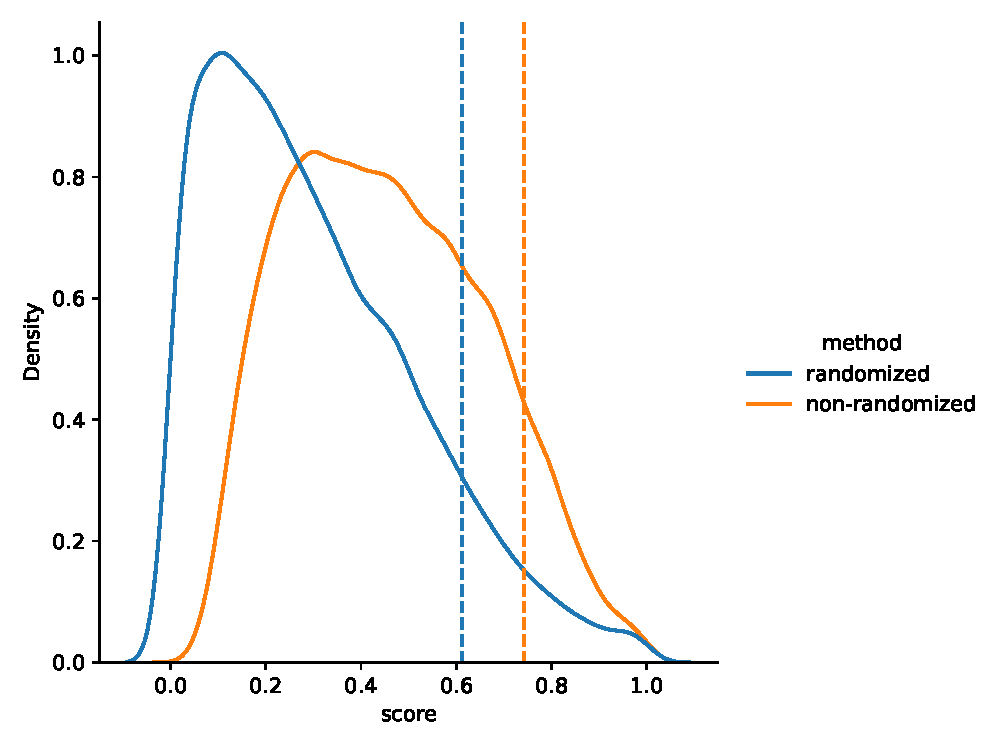
\includegraphics[width=\linewidth]{graphConformal/figures/aps_dist}
    \end{subfigure}
    \begin{subfigure}{0.7\linewidth}
        \centering
        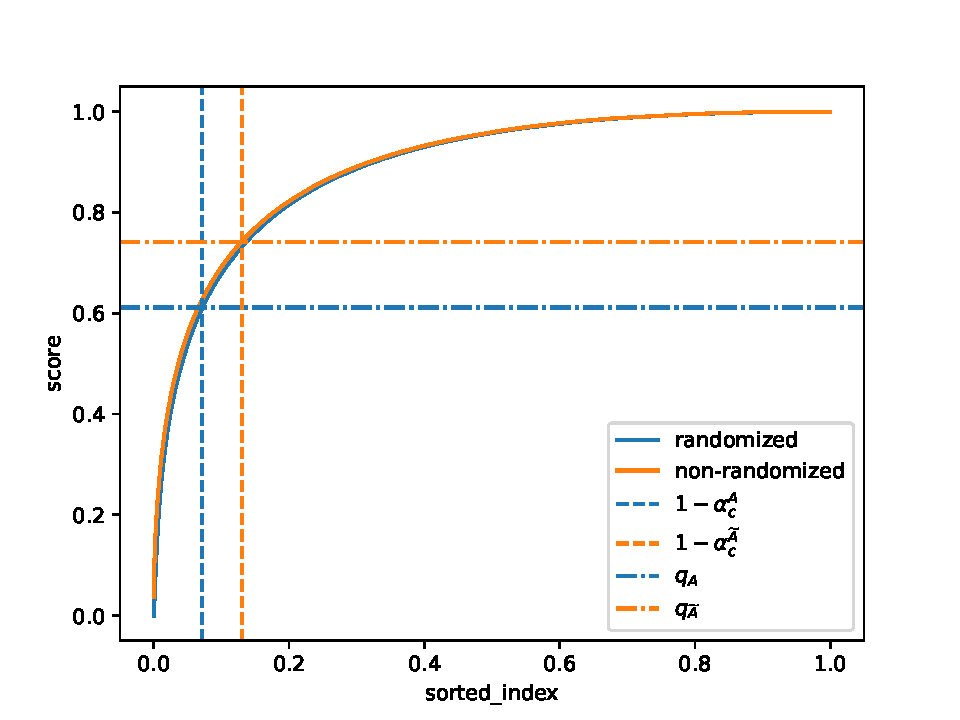
\includegraphics[width=\linewidth]{graphConformal/figures/aps_sorted}
    \end{subfigure}
    \caption{Figure showing the scores for an example dataset. (top) shows the shift in the quantile for $A$ and $\Tilde{A}$ for the correct class. (bottom) shows the shift $\alpha_c$ for $A$ and $\Tilde{A}$ using scores $A'$ for the incorrect classes.}
    \label{fig:APS:efficiency}
\end{figure}

%\pmcomment{empirical quantiles with epsilon}

%\begin{align*}
%   |S(\vx_{n+1}, u; \hat{\pi}, \tau_A)| - |\Tilda{S}(\vx_{n+1}; \hat{\pi}, \tau_{})|
%\end{align*}

\subsection{Notes on Transductive NAPS}
Neighborhood Adaptive Prediction Sets (NAPS) can construct predictive sets via Conformal Prediction under relaxed exchangeability (or non-exchangeability) assumptions~\cite{barber2023conformal}.
In the context of graphs, NAPS was initially implemented in the inductive setting~\cite{clarkson2023distribution}.
However, it can be used in the transductive setting as well~\cite{zargarbashi23conformal}. 
NAPS in the transductive setting is based on APS where $s_i = A(\vx_i, y_i, u_i;\hat{\pi}_i)$, or $A(\vx_i, y_i;\hat{\pi}_i)$ (depending on whether the randomized version is used), is computed for each node in $\gD_{\text{calib}}$. 
Using these scores, a weighted quantile is computed to produce the score threshold for prediction sets (Equation~\ref{eq:NAPS:quantile})
Unlike APS, the quantile is defined by placing weighted point masses ($\delta$) at each score from the calibration set under consideration for quantile computation.
The point mass at $+\infty$ indicates that the score for test node $n+1$ is unknown (and unbounded due to non-exchangeability), and thus, a point mass at the maximum value ($+\infty$) is required.%\ascomment{I want to state the intuitive reason for the infinite point mass since it was not clearly stated in the NAPS paper.} 
\begin{align}
    \hat{q}^{\text{NAPS}}_{n+1} = \text{Quantile}\bigg(1-\alpha, \bigg[\sum_{i\in\gD_{\text{calib}}}\Tilde{w}_{i}\cdot \delta_{s_{i}}\bigg] + \Tilde{w}_{n+1}\cdot \delta_{+\infty}\bigg)
    \label{eq:NAPS:quantile}
\end{align}

For NAPS to produce viable prediction sets, the weights, $w_i\in [0,1]$, for nodes under consideration in the calibration set must be chosen in a data independent fashion, i.e., they cannot leverage the feature vectors associated with the calibration nodes~\citep{barber2023conformal}.
NAPS leverages the graph structure to assign these weights, assigning non-zero weights to nodes within a k-hop neighborhood $\gN_{n+1}^k$ of the test node $v_{n+1}$.
%Since exchangeability is not assumed, a weight function leveraging graph homophily can be used to produce weights, $w_i\in [0,1]$, for nodes in the calibration set \cite{barber2023conformal}. 
The three implemented weight functions are uniform, $w_u(d_i) = 1$, hyperbolic $w_h(d_i) = \frac{1}{d_i}$, and exponential, $w_e(d_i) = 2^{-d_i}$ for nodes in the k-hop neighborhood, where $d_i$ is the distance from $v_{n+1}$ to $v_i \in \gV_{\text{calib}}$.
Formally, the weight function for each node, $v_i \in \gV_{\text{calib}}$ can be seen in Equation \ref{eq:NAPS:weight} below, where $w_x(d_i)$ is the selected weight function.
These weights are then normalized to compute $\Tilde{w}_i$ such that $\sum_{i\in\gD_{\text{calib}}} \Tilde{w}_i + \Tilde{w}_{n+1} = 1$ \cite{barber2023conformal}.
\begin{align}
    w_i = \begin{cases}
w_x(d_i), & i\in \gD_{\text{calib}}\cap\mathcal{N}_{n+1}^k\\
0,& i\in \gD_{\text{calib}}\setminus\mathcal{N}_{n+1}^k
\end{cases}
    \label{eq:NAPS:weight}
\end{align}

Using the NAPS quantile, $\hat{q}^{\text{NAPS}}_{n+1}$, the prediction sets can be constructed similarly to other Conformal Prediction algorithms.
Note that NAPS was originally designed for the inductive setting; transductive differs as non-zero weights are assigned to fewer nodes as only a subset of the graph nodes are assigned to be calibration nodes.
In the inductive setting, no exchangeability cannot be assumed and the entire graph prior to the test phase is considered as a calibration set leading to a larger number of non-zero weights.

\noindent \textbf{NAPS Implementation}
NAPS is computationally more expensive with regard to time and memory as a k-hop intersection must be computed for each test node.
We optimized this implementation using a batched approach that works with sparse tensors (Algorithm \ref{alg:NAPS:Quantile}).
Informally, the test nodes are first split up into batches. 
Then, for each batch, the distance to each node in the k-hop neighborhood is computed.
Following this, the weights function for the corresponding nodes are computed before computing the quantile for each node.
The batched approach ensures that sufficient memory is available for the necessary computations - especially for computing the distance to each node in the k-hop neighborhood without needing to densify a sparse graph.

\begin{algorithm}
\caption{NAPS Quantile Implementation}\label{alg:NAPS:Quantile}
\begin{algorithmic}[1]
\Procedure{NAPS\_Quantile}{$w,k,\calib,\test,\mathcal{D},\mathcal{S}_{\text{calib}},b,\alpha$}
    \State $\{\mathcal{B}_1,\mathcal{B}_2,\hdots,\mathcal{B}_b\}\gets \Call{\text{split}}{\test,b}$ \Comment{Split test nodes into b batches}
    \State $q\gets \Call{\text{zeros}}{\test,1}$\Comment{$q\in \mathbb{R}^{|\test| \times 1}$}
    \For{$\mathcal{B}_n \in \{\mathcal{B}_1,\mathcal{B}_2,\hdots,\mathcal{B}_b\}$}
        \State $\text{k\_hop} \gets \Call{\text{Sparse\_k\_hop}}{k,\mathcal{B}_n,\calib,\mathcal{D}}$\Comment{k\_hop $\in \mathbb{R}^{|\mathcal{B}_n|\times|\calib|}$}
        \State $\text{weights}\gets \Call{\text{compute\_weights}}{w,\text{k\_hop}}$\Comment{weights $\in \mathbb{R}^{|\mathcal{B}_n|\times|\calib|}$}
        \State $q[\mathcal{B}_n]\gets \Call{\text{compute\_quantile}}{1-\alpha,\text{weights},\mathcal{S}_{\text{calib}}}$
    \EndFor\label{NAPSquantileendwhile}
    \State \textbf{return} $q$\Comment{Return the quantiles for each test node}
\EndProcedure
\end{algorithmic}
\end{algorithm}

To ensure scalability for large graphs, all the computations until the quantile computation setep were done via sparse tensors. 
Algorithm \ref{alg:NAPS:SparseKHop} illustrates how the distance to each calibration node in the k-hop neighborhood can be computed via  sparse tensorr primitives.
The sign function based formulation uses the fact that subtracting $n+1$-hop paths from a matrix containing up to $n$ hops to ensure negative values at paths of length exactly $n+1$, with the rest being 0.
%To ensure that the minimum distance to nodes in the k-hop neighborhood is reported, the sign function is applied to the matrix containing paths exactly n hops away. This is subtracted from the matrix containing distances up to n-1 hops. A value can only be less than 0 after this subtraction if the corresponding index in the matrix containing distances up to n-1 hops was 0. Using this, the nodes that are at a minimum n hops away can be identified and added to the matrix containing distances to calibration nodes in the k-hop neighborhood. The described calculations can be done using sgn, and signbit (to check if an element is negative) in PyTorch.\ascomment{Shorted this paragraph}  

\begin{algorithm}
\caption{Sparse K Hop Neighborhood Implementation}\label{alg:NAPS:SparseKHop}
\begin{algorithmic}[1]
\Procedure{Sparse\_k\_hop}{$k,\mathcal{B},\calib,\mathcal{D}$}
    \State $\text{A}\gets \Call{\text{Get\_Adjacency}}{\mathcal{D}}$ \Comment{Adjacency of $\mathcal{D}$, A $\in \mathbb{R}^{|\mathcal{D}|\times|\mathcal{D}|}$}
    \State $\text{path\_n}\gets \text{A[$\mathcal{B},:$]}$\Comment{path\_n $\in \mathbb{R}^{|\mathcal{B}|\times|\mathcal{D}|}$ }
    \State $\text{k\_hop}\gets \text{path\_n[$:,\calib$]}$\Comment{k\_hop $\in \mathbb{R}^{|\mathcal{B}|\times|\calib|}$ }
    \For{$n \in \{2,3,\hdots,k\}$}
        \State $\text{path\_n} \gets (\text{path\_n})\text{A}$
        \State $\text{neg\_if\_n}\gets \text{k\_hop}-\Call{\text{sgn}}{\text{path\_n[$:,\calib$]}}$\Comment{negative value $\implies$ n hops away}
        \State $\text{in\_n\_hop}\gets (\text{neg\_if\_n}<0)\times n$ \Comment{Nodes that are a min distance of n}
        \State $\text{k\_hop} \gets \text{k\_hop} + \text{in\_n\_hop}$
    \EndFor\label{khopendwhile}
    \State \textbf{return} $\text{k\_hop}$\Comment{$\forall_{i,j}\, \text{\textbf{If} dist($i,j$)}  \leq k \text{ \textbf{then} k\_hop[$i,j$]} = \text{dist}(i,j), \text{\textbf{else} k\_hop[$i,j$]}=0$}
\EndProcedure
\end{algorithmic}
\end{algorithm}

\subsection{Diffusion Adaptive Prediction Sets}
The Diffusion Adpative Prediction Sets (DAPS) approach for conformal node classification on graphs was introduced by \citet{zargarbashi23conformal}.
The intuition behind DAPS is that the prevalence of homophily in graphs implies that the non-conformity scores for two connected scores should be related.
DAPS uses a diffusion step to capture this relationship and uses the non-conformity scores modified by diffusion to generate the prediction sets.
Formally, suppose $s(v, y)$ is a point wise non-conformity score for a node $v$ and label $y$ (e.g., TPS or APS)
\[
    \hat{s}(v, y) = (1 - \lambda) s(v, y) + \frac{\lambda}{|
    \gN_v|} \sum\limits_{u \in \gN_v} s(u, y)
\]
where $\gN_v$ is the 1-hop neighborhood of $v$ and $\lambda \in [0, 1]$ is a hyperparameter controlling the diffusion.

\citet{zargarbashi23conformal} use the APS score as the point wise score in diffusion process as it is adaptive and uniformly distribution in $[0, 1]$ under oracle probability.
However, as we noted earlier, using class wise thresholds provides a mechanism to produce adaptive scores from TPS as well.
Thus, we create DTPS, a variation of DAPS using TPS-Classwise scores as the point wise scores in the diffusion process.

\subsection{Conformalized GNN}
\begin{figure}
    \centering
    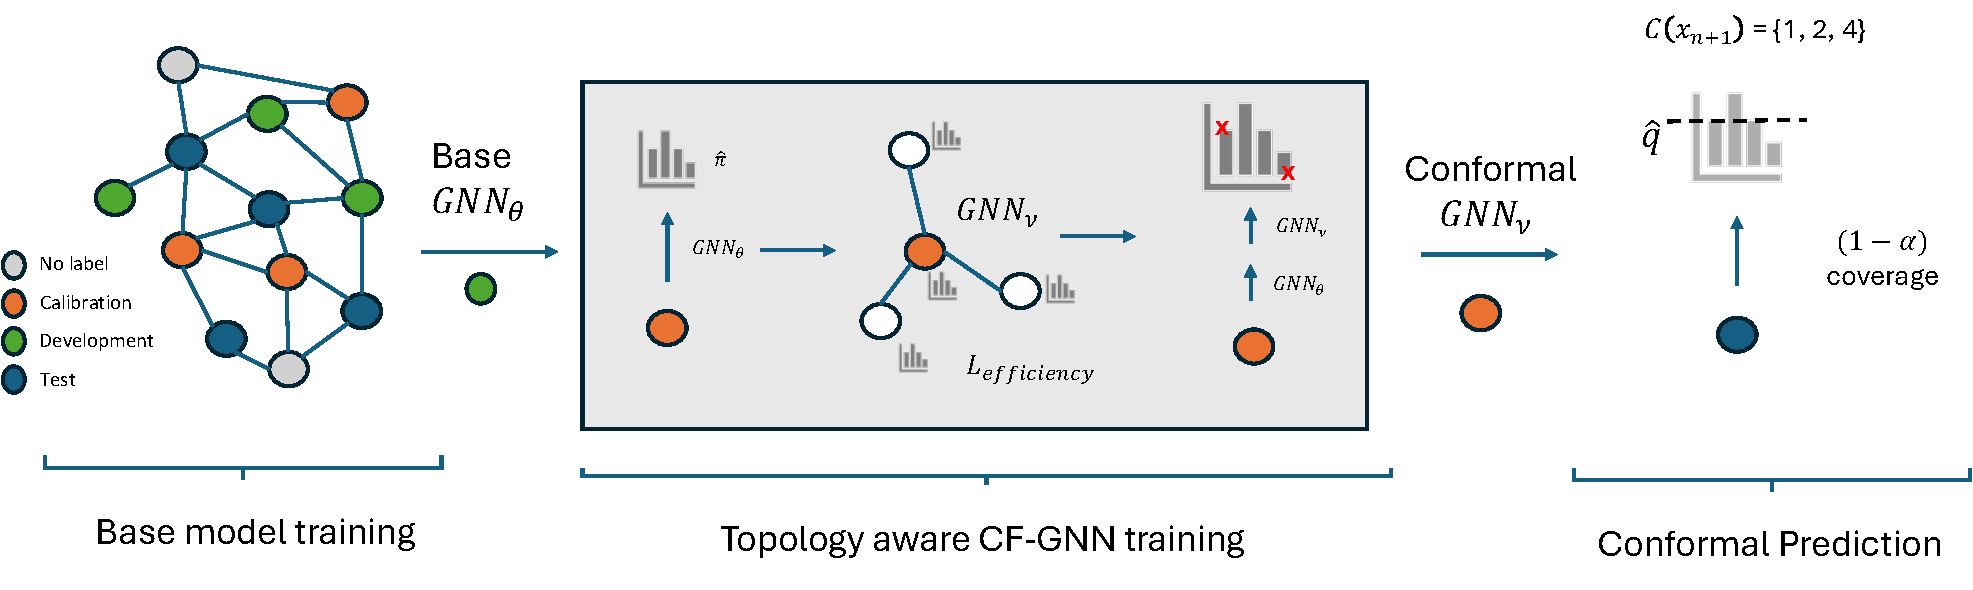
\includegraphics[width=\linewidth,alt={CF-GNN three stage training procedure.}]{graphConformal/figures/CFGNN.pdf}
    \caption{Procedure for training CF-GNN. First (left), the base model is trained on the training set. Then, (middle) the CF-GNN is trained to maximize efficiency over the calibration set. Finally , (right) the non-conformity scores from the combined models are used to generate the prediction sets.}
    \label{fig:conformalized_gnn}
\end{figure}

Conformalized GNN (CFGNN)~\citep{huang2024uncertainty} is a GNN-based approach for conformal prediction.
The authors observed that inefficiencies are correlated between nodes having similar neighborhood topology in a graph setting.
They use a GNN during the calibration phase, which is trained to correct the scores output from the base model such that the corrected scores maximize the efficiency of the conformal prediction.
For classification-based losses, CFGNN utilizes the fact that all steps in the conformal prediction stage for computing the prediction sets (non-conformity score computation, quantile computation, thresholding) can be expressed as differentiable operations.
Thus, a GNN can be trained directly using efficiency as a loss function.
Figure~\ref{fig:conformalized_gnn} provides a high-level overview of the CFGNN approach.

\noindent \textbf{CFGNN Implementation Improvements}
The choice of the conformal loss during calibration and test plays an important role in determining the overall performance of the CFGNN.
\citet{huang2024uncertainty} use a TPS loss for the calibration phase and the non-randomized APS loss for constructing the final prediction sets.
Our preliminary experiments (Figure~\ref{fig:CFGNN:preliminary}) with replacing the APS loss with a randomized version demonstrated that these losses must be tuned carefully to ensure that the CFGNN is able to improve upon the base models non-conformity scores.
Some improvements shown in CFGNN (Figure~\ref{fig:CFGNN:preliminary}, right) get nullified when the randomized APS loss is used (left).

Additionally, CFGNN uses full batch training which makes it unable to scale for larger graphs.
We implemented a batched version of CFGNN to ensure that it can be used for larger graphs.
Finally, to speed up computation, we allow the use of cached outputs from the base model rather than having to sample neighbors for both the base model and the CFGNN.
Algorithm~\ref{alg:cfgnn:catching} shows these improvements in the CFGNN implementation.
We cache the output of the base $\text{GNN}_\theta$ prior to running the CFGNN training loop, allowing the sampling of $m$ layers of message passing graphs rather than $m + l$ layers required by the baseline CFGNN.
In addition, we control the batch size $b$ when sampling neighbors.
These changes significantly speeds up the computation for CFGNNs (see Section~\ref{sec:conformal:results:cfgnn:runtime} for speedup results).
\begin{algorithm}
    \caption{CFGNN batching + caching implementation}\label{alg:cfgnn:catching}
    \begin{algorithmic}[1]
    \State $\text{GNN}_{\theta}$ \Comment{$l$ layer base GNN, with pretrained, fixed weights}
    \State $\text{GNN}_{\phi} \gets \Call{\text{RandomInitialization}}{\phi}$ \Comment{$m$ layer trainable CFGNN}
    \If{cache\_base}
        \State $\gX \gets \text{GNN}_{\theta}(\gG, \gX)$ \Comment{Compute base model output}
    \EndIf
    \Procedure{CFGNNTrainStep}{$\calib, \gG, \gX$}
        \State $\gB \gets \Call{\text{SampleBatch}}{\calib, b}$ \Comment{batch size $b$ is $|\calib|$ for base CFGNN}
        \If{cache\_base}
            \State{$\text{CFFeats, CFMsgGraphs} \gets \Call{\text{ NeighborSampler}}{\gB, m, \gX}$}
        \Else
            \State{$\text{Feats, MsgGraphs} \gets \Call{\text{NeighborSampler}}{\gB, l + m, \gX}$}
            \State{$\text{CFFeats} \gets \text{GNN}_\theta(\text{Feats}, \text{MsgGraphs}_{0, \dots, m-1})$}
            \State{$\text{CFMsgGraphs} \gets \text{MsgGraphs}_{m, \dots, m+l-1}$}
        \EndIf
        \State $\text{scores} \gets \text{GNN}_{\phi}(\text{CFFeats}, \text{CFMsgGraphs})$
        \State $\gL \gets \Call{\text{ConformalLoss}}{\text{scores}, \gB}$
        \State $\Call{\text{UpdateWeights}}{\text{GNN}_\phi, \gL}$
    \EndProcedure
    \end{algorithmic}
\end{algorithm}


\begin{figure}
    \centering
    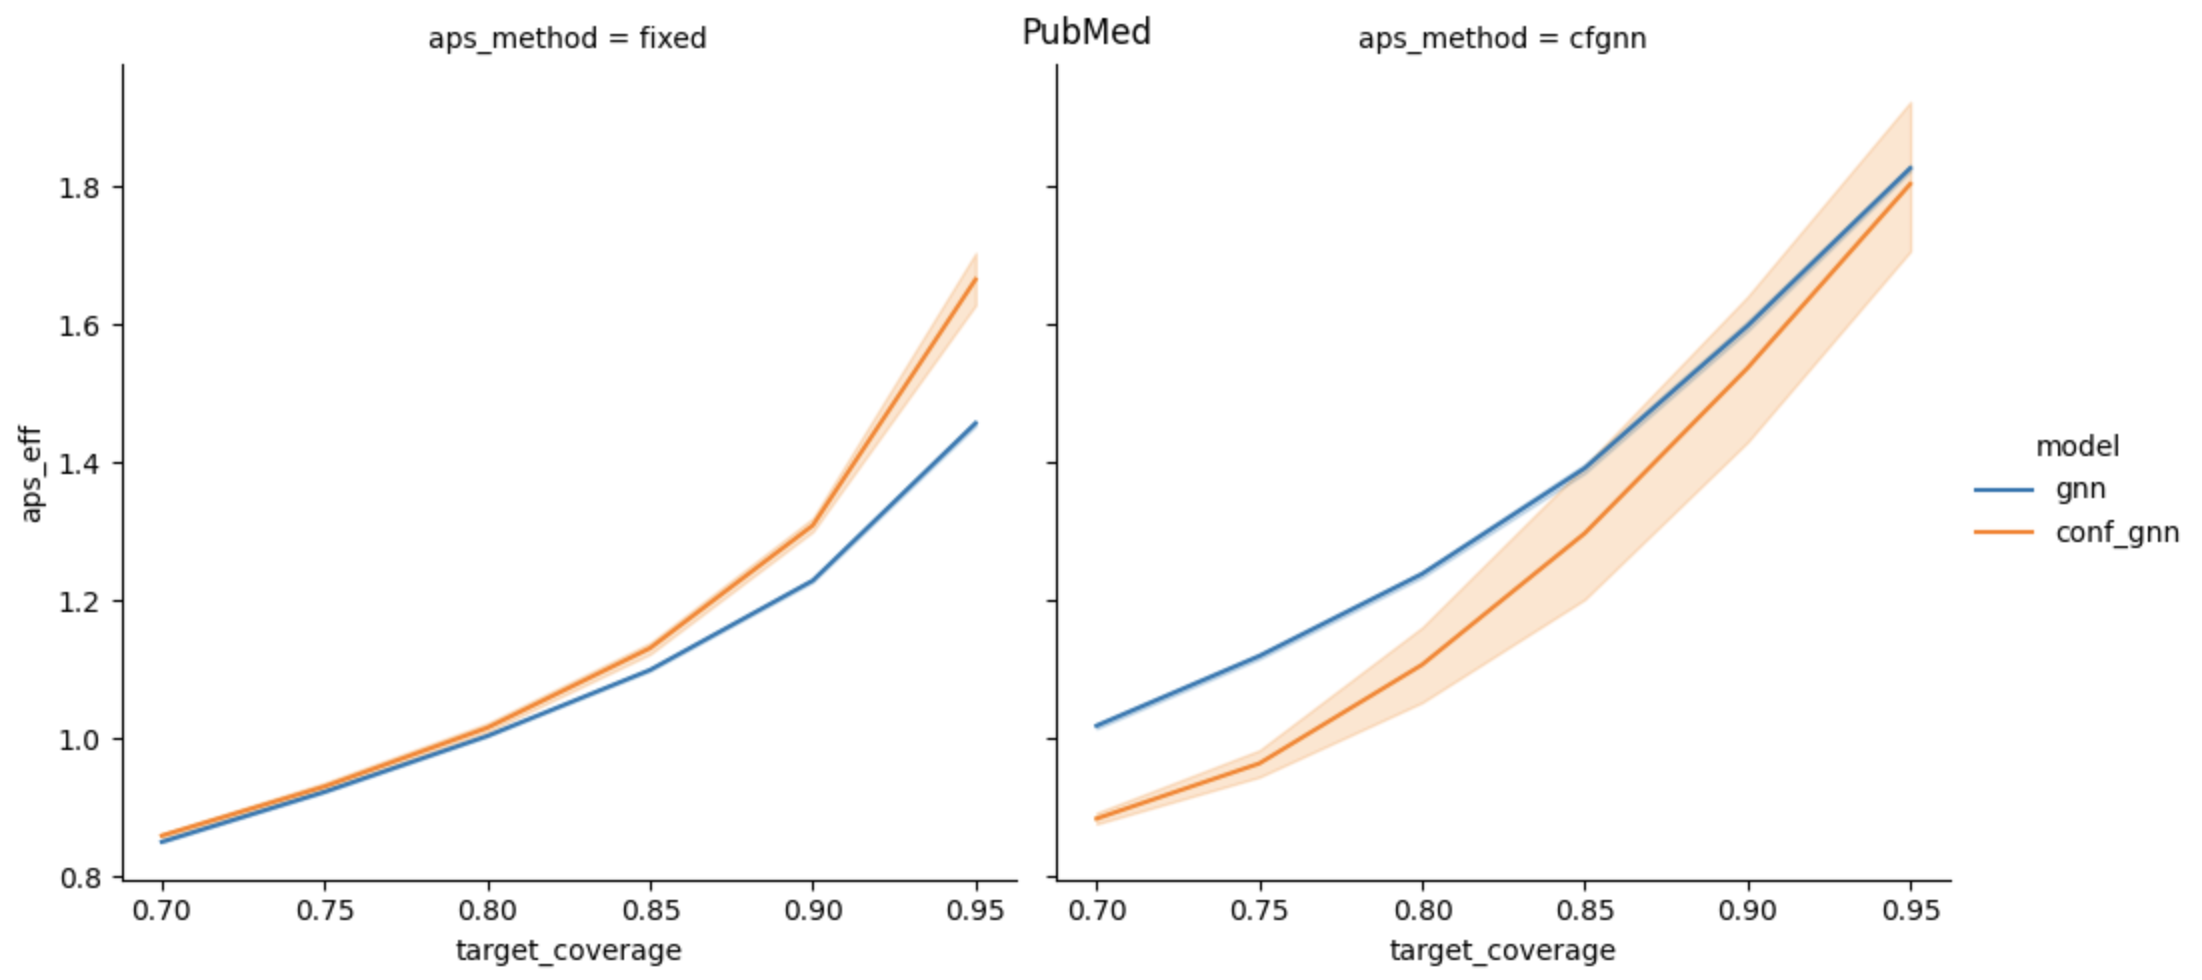
\includegraphics[width=0.8\linewidth,alt={Preliminary results on effciency comparison with APS vs CFGNN.}]{graphConformal/figures/PubMed_CF.png}
    %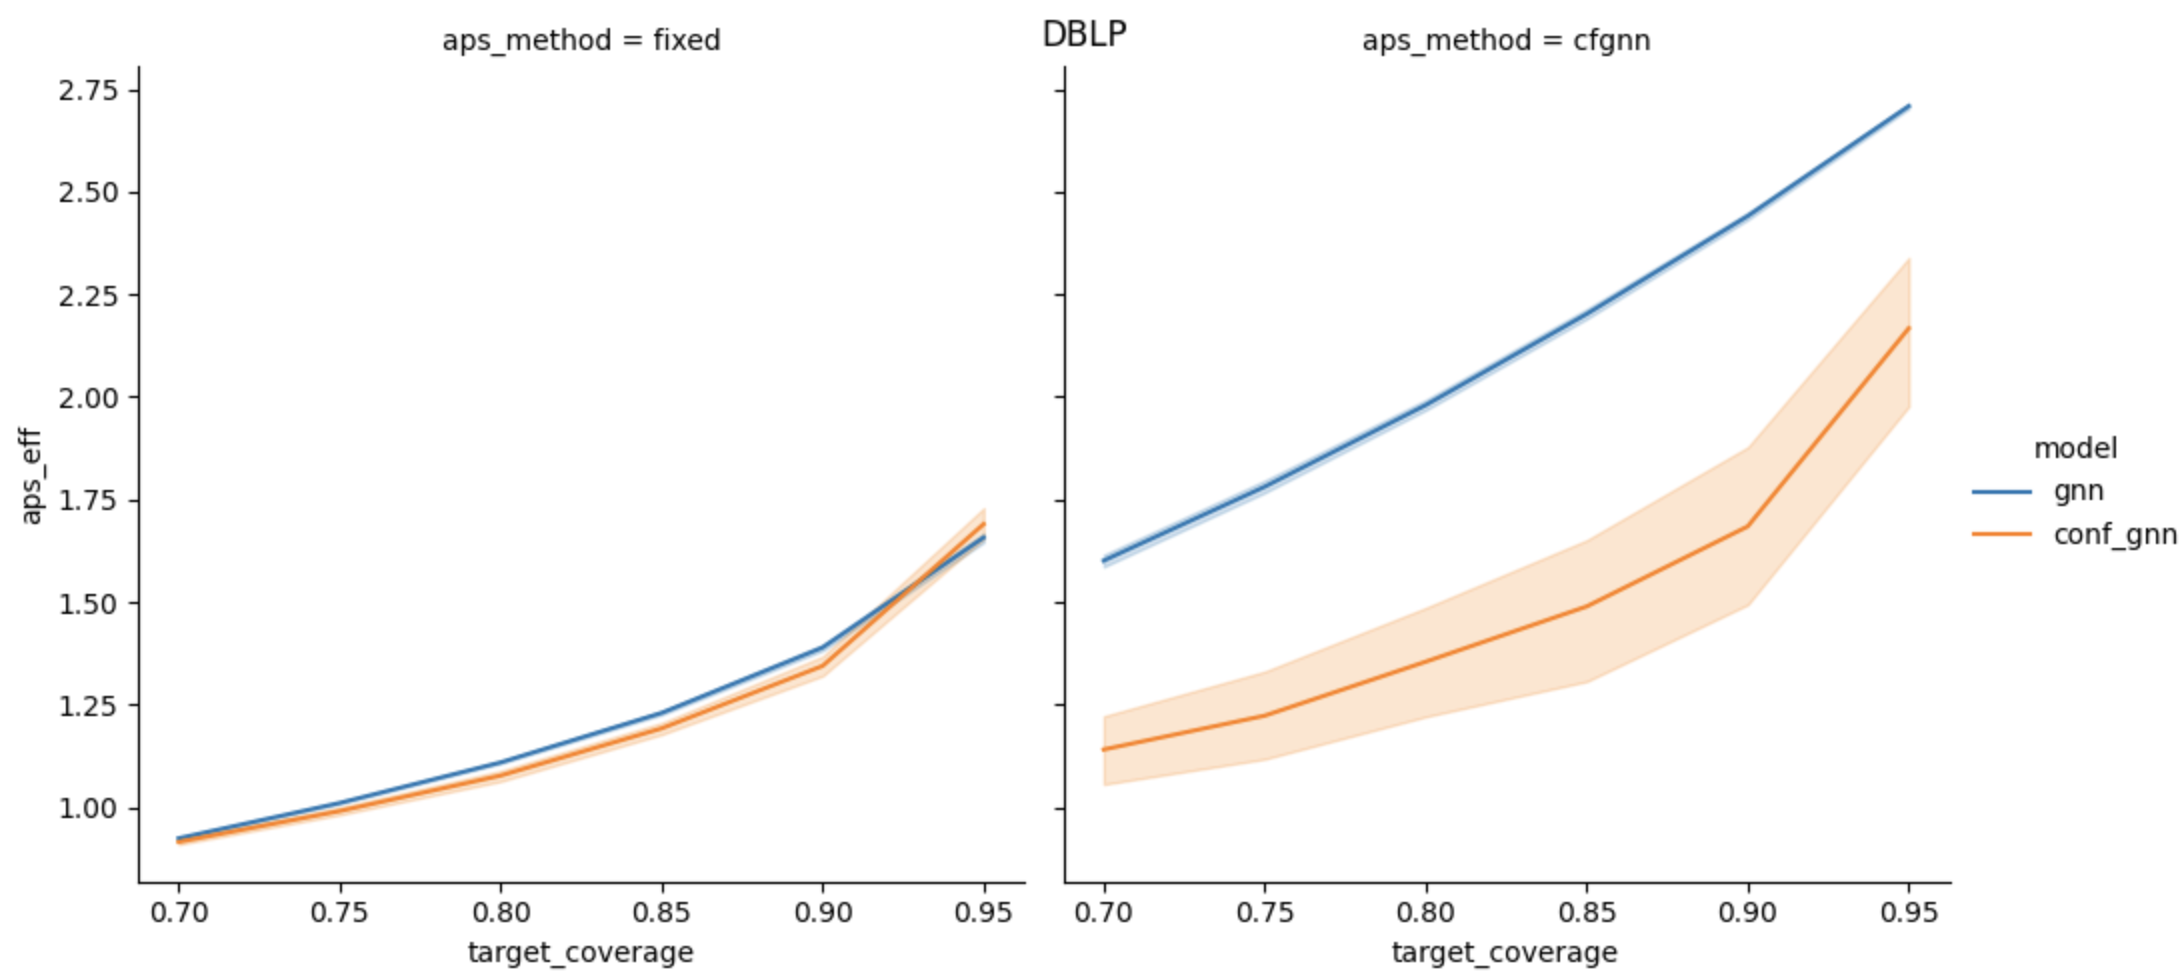
\includegraphics[width=0.7\linewidth]{graphConformal/figures/DBLP_CF.png}
    \caption{Comparing the efficiency (average output set size) for the base model and the CFGNN on the Pubmed dataset. The plot on the left uses the fixed version of the APS score (with randomized sets) while on the right uses the non-randomized version.}
    \label{fig:CFGNN:preliminary}
\end{figure}



\section{Evaluation of Graph Conformal Prediction}
\subsection{Datasets}

\begin{table}
    \centering
    \begin{tabular}{ccccc}
        \toprule
        Dataset & Nodes & Edges & Classes & Features \\
        \midrule
        CiteSeer & 3,327 & 9,228 & 6 & 3,703 \\ 
        Amazon\_Photos & 7,650 & 238,163 & 8 & 745 \\
        Cora & 19,793 & 126,842 & 70 & 8,710 \\
        PubMed & 19,717 & 88,651 & 3 & 500 \\
        Coauthor\_CS &  18,333 & 163,788 & 15 & 6,805 \\
        Coauthor\_Physics & 34,493 & 495,924 & 5 & 8,415 \\
        \bottomrule
    \end{tabular}
    \caption{Summary statistics for Datasets chosen for evaluation.}
    \label{tab:conformal:datasets}
\end{table}


We selected datasets of varying sizes to evaluate the performance of the graph conformal prediction methods.
For the citation datasets, the nodes are publications, and the edges denote citation relationships.
Features are bag-of-words representations of the documents.
The task is to predict the category of each publication.
\textbf{CiteSeer} is a citation network dataset designed for the node classification task, with nodes as publications and edges denoting citation relationships.
\textbf{Amazon\_Photos} is a segment of the Amazon co-purchase graph~\cite{mcauley2015image} where nodes represent goods, edges represent goods frequently bought together, features are bag-of-words representations of product reviews, and the task is to predict the category of each good.
\textbf{Cora} We use CoraFull~\cite{shchur2018pitfalls}, an extended version of the common Cora citation network dataset.
Summary statistics for the datasets are provided in Table~\ref{tab:conformal:datasets}.
The objective is to predict the category of each node (publication).
\textbf{PubMed} is a citation network dataset designed for the node classification task, with nodes as publications and edges denoting citation relationships. The goal is to predict the category of each node (publication).
For all chosen datasets, we used the version provided by the Deep Graph Library~\cite{wang2019dgl}.
\textbf{Coauthor\_CS} and \textbf{Coauthor\_Physics} are co-authorship graphs extracted from the Microsoft Academic Graph and used for KDD Cup 2016. In this dataset, nodes are authors and edges denoting co-authorship relationships. The task is to predict the most active field of study for each author.

To help characterize the behavior of different approaches, we categorize these into sizes based on the number of nodes, with \textbf{Cora} and \textbf{Amazon\_Photos} designated as small (S), \textbf{CiteSeer}, \textbf{PubMed}, and \textbf{Coauthor\_CS} as medium (M), and \textbf{Coauthor\_Physics} as large (L).

\subsection{Metrics}
We evaluate the following metrics for the graph conformal prediction methods:
\begin{itemize}
    \item \textbf{Coverage:} The proportion of test instances for which the true label is contained in the prediction set.
    \item \textbf{Efficiency:} The average size of the prediction set.
    \item \textbf{Label Stratified Coverage:} The mean of coverage for each class. This metric is useful for understanding whether a method is adaptive and has balanced coverage for different classes.
    \item \textbf{Size Stratified Coverage:} The mean of coverage across different sizes of prediction sets. This metric is useful for understanding whether a method is adaptive and does not under/over cover hard/easy samples.
    %\item \textbf{Size Stratified Coverage Violation:} Measures the maximum deviation from the coverage goal across different prediction set sizes. 
    \item \textbf{Singleton Hit Ratio:} The proportion of test instances for which the true label is the only label in the prediction set. This metric measures the frequency with which a method does not require generation of a prediction set having multiple labels.
\end{itemize}

\subsection{Methods}
We discussed the theoretical and empirical tradeoffs of different methods in Section~\ref{chp:graphConformal:sec:conformal_scores_tradeoffs}.
For completeness, we list all the methods that we compare here.
\textbf{Threshold Prediction Sets}~\cite{sadinle2019least}, with two variants, TPS and TPS-Classwise (using class wise thresholds for adapting to class imbalance).
\textbf{Adaptive Prediction Sets}~\cite{romano2020classification} with two variants, APS and APS-Randomized (using the uniform random quantile adjustments).
\textbf{Regularized Adaptive Prediction Sets}~\cite{angelopoulos2021uncertainty}, a variation of APS with a regularization term to ensure that the prediction sets are not too large.
\textbf{Diffused Adaptive Prediction Sets}~\cite{zargarbashi23conformal}, with two variations DAPS and DTPS, which uses a diffusion process over TPS-Classwise.
\textbf{Normalized Adaptive Prediction Sets}~\cite{clarkson2023distribution} with three variations corresponding to the weighing function used.
\textbf{CF-GNN}~\cite{huang2024uncertainty}, a GNN based approach for conformal prediction. We label the original implementation of CFGNN as CFGNN-Original and our improved implementations as CFGNN-APS (using randomized APS as the loss function for training/evaluation) and CFGNN-TPS (using TPS as the loss function for training/evaluation).

%\subsection{Notes on Parameter Tuning and Evaluation}
%\pmcomment{TODO for final version}

\subsection{Results}

\subsubsection{Full-Split (FS) Partitioning}

\begin{figure}
    \centering
    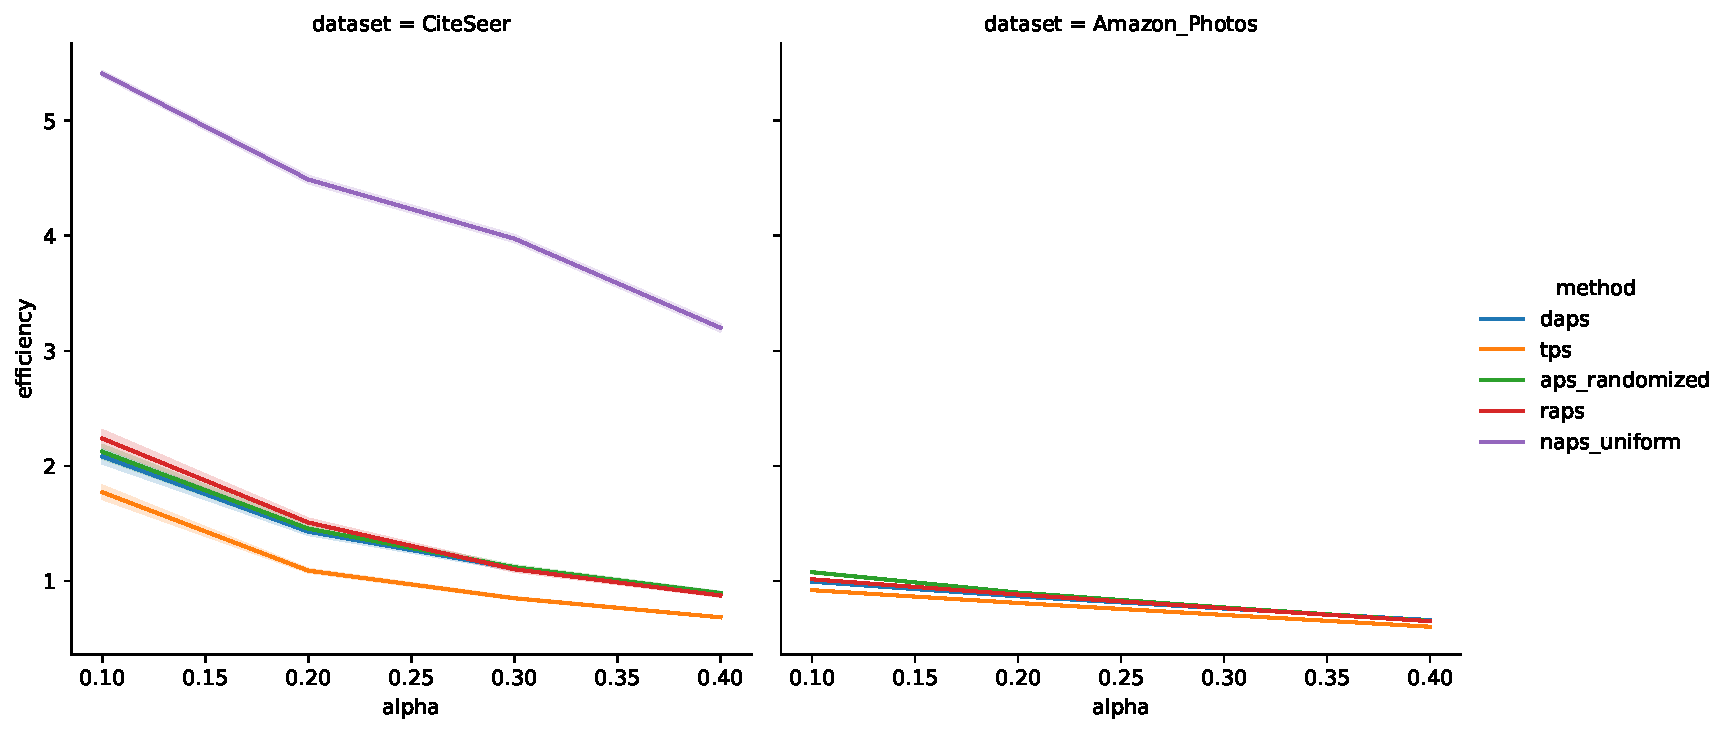
\includegraphics[width=\linewidth]{graphConformal/figures/split/small_datasets_efficiency.pdf}
    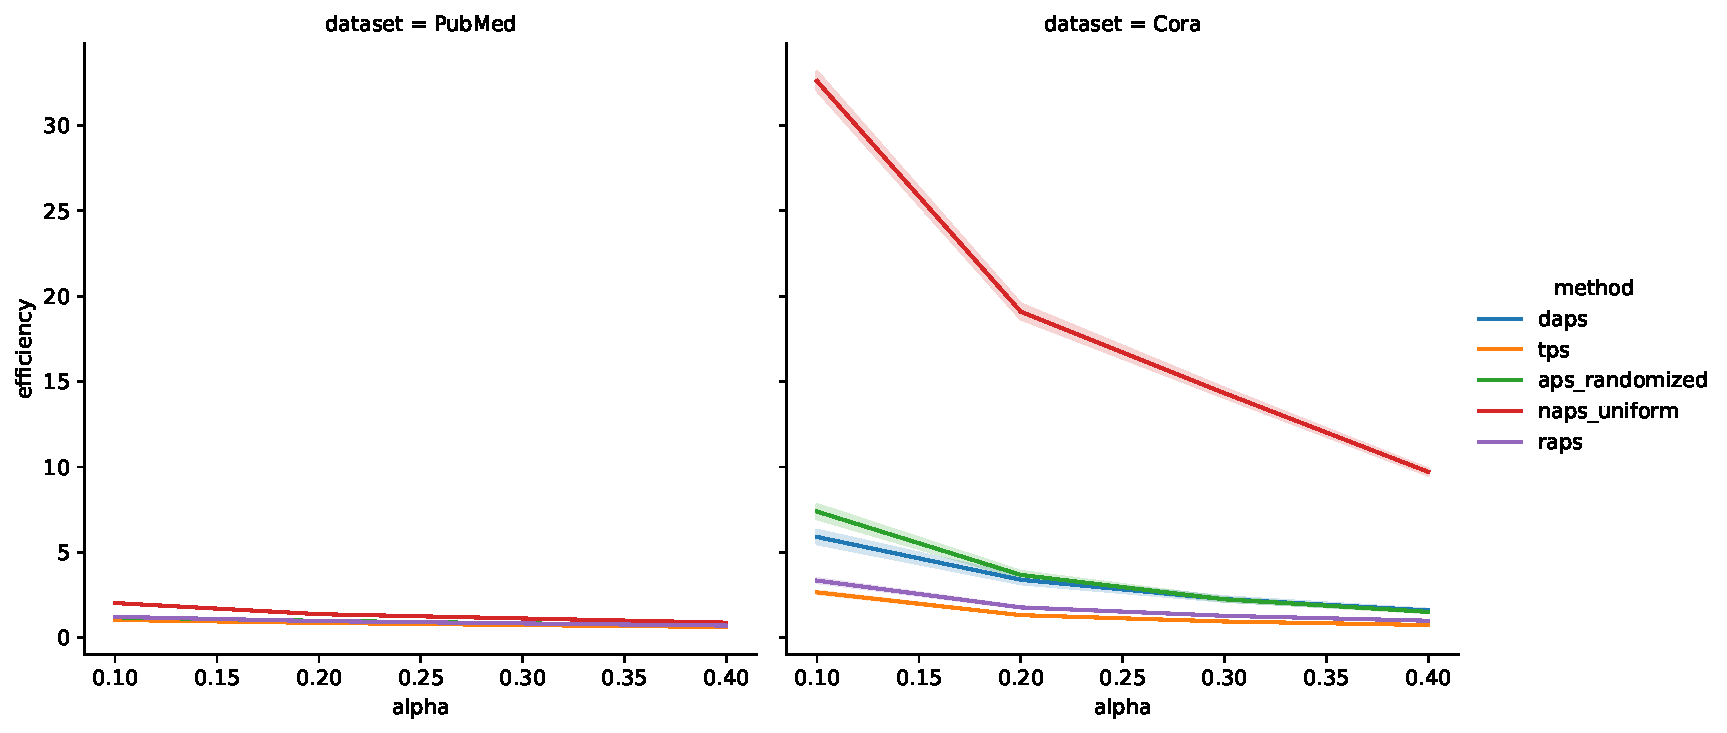
\includegraphics[width=\linewidth]{graphConformal/figures/split/med_1_datasets_efficiency.pdf}
    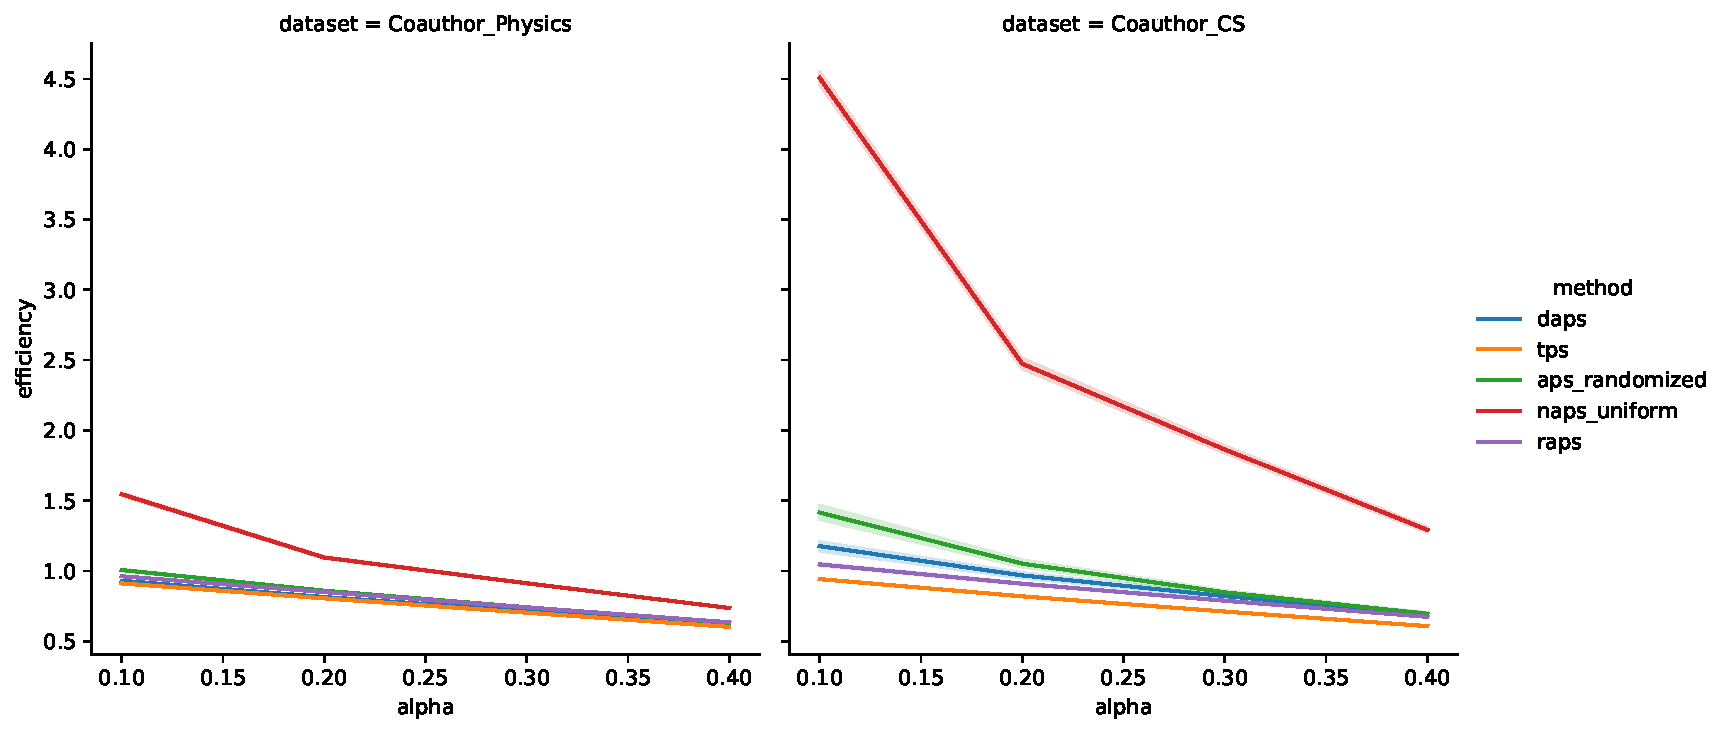
\includegraphics[width=\linewidth]{graphConformal/figures/split/med_2_datasets_efficiency.pdf}
    \caption{Plots for efficiency vs $\alpha$ for the major methods across the all the datasets. TPS consistently has the best efficiency }
\end{figure}





\begin{subappendices}
    \section{Optimal $\tau$ for APS}
\label{appx:APS:tau}
For simplicity, assume that the probabilities are distinct.

From the definition of $A$ \eqref{eq:APS:score}
\begin{align*}
    A(\vx, y, u;\hat{\pi}) &= \min\{\tau \in [0, 1]: y \in S(\vx, u; \hat{\pi}, \tau)\}
\end{align*}
Define 
\[
\Sigma_{\hat{\pi}}(\vx, m) = \sum\limits_{i=1}^m \hat{\pi}_{(i)}(\vx)
\]
From the definition of $S(\vx, u; \hat{\pi}, \tau)$ from \eqref{eq:APS:S}, conisder the following cases:

\textbf{Case 1:} $\tau = \Sigma_{\hat{\pi}}(\vx, r_y)$, then $L(x; \hat{\pi}, \tau) = y$ and thus, $V(\vx; \pi, \tau) = 0$.
Thus $\Pr[u > V(\vx; \pi, \tau)] = 1$ and hence, $P[y \in S(\vx, u; \hat{\pi}, \tau)] = 1$.

\textbf{Case 2:} $\tau = \Sigma_{\hat{\pi}}(\vx, r_y-1)$, then $y \not\in S(\vx, u, \hat{\pi}, \tau)$ in either case, since only classes with $\hat{\pi}_i(\vx) > \hat{\pi}_y(\vx)$ could be included. \pmcomment{This is the edge case where tie breaking is required for a completely general proof.}

\textbf{Case 3:} $\tau = \Sigma_{\hat{\pi}}(\vx, r_y) - \varepsilon \hat{\pi}_y$.
Then we have $L(x; \hat{\pi}, \tau) = y$ again, and 
\begin{align*}
    V(\vx; \pi, \tau) &= \frac{1}{\hat{\pi}_y(\vx)}\left\{ \left[ \sum_{j=1}^{r_y} \hat{\pi}_{(j)}(\vx) \right] - \tau \right\} \\
                      &= \frac{1}{\hat{\pi}_y(\vx)}\left\{ \left[ \sum_{j=1}^{r_y} \hat{\pi}_{(j)}(\vx) \right] - (\Sigma_{\hat{\pi}}(\vx, r_y) - \varepsilon \hat{\pi}_y) \right\}\\
                      &= \varepsilon
\end{align*}
For $y$ to be included in $S(\vx, u; \hat{\pi}, \tau)$, we would require that $u \geq V(\vx; \pi, \tau)$, i.e., $u \geq \varepsilon$. 
We want the minimal $\tau$, which is equivalent to maximizing $\varepsilon$. 
Thus, $\tau = \Sigma_{\hat{\pi}}(\vx, r_y) - u \hat{\pi}_y$ is the required solution.

\subsection{Non-randomized set}
The inclusion criterion for the score given the threshold $\tau$ is $\Tilde{A}(\vx, y; \hat{pi}) \leq \tau$

To include the currct label $y_i$ while minimizing the chosen threshold $\tau$, we would require $\tau = \sum\limits_{j=1}^{r_{y_i}} \hat{\pi}_{(j)}(\vx)$ 
\end{subappendices}
